
\section{Finding \smu{} Usage Patterns} \label{sec:methodology}

We examined the artifacts in the Maven Central software repository to identify usage patterns for \unsafe{}.
This section describes our methodology for identifying these patterns. 

\begin{figure}[h!]
\includegraphics[page=6,width=\columnwidth]{chapters/unsafe/artifacts}
\caption{\artexp{com.lmax}{disruptor} call sites}
\label{fig:appartfingerprint}
\end{figure}

\begin{figure}[h!]
\includegraphics[page=5,width=\columnwidth]{chapters/unsafe/artifacts}
\caption{\artexp{org.scala-lang}{scala-library} call sites}
\label{fig:langartfingerprint}
\end{figure}

Our first step is to visualize how an artifact uses \unsafe{}.
To this end, we count the \unsafe{} call sites and field usages per class in each artifact.
Figures~\ref{fig:appartfingerprint} and \ref{fig:langartfingerprint} show two examples of call sites usages for \artexp{com.lmax}{disruptor} and \artexp{org.scala-lang}{scala-library} respectively.
Each row shows a fully qualified class name and their usage of \smu{}.

After determining the call sites and field usage per artifact, we tried to find a way to group artifacts by how they use \smu{}.
The first issue is to determine which method calls work together to achieve a goal.
These calls might all be located within a single class, be spread across different classes within a package, or be spread across different packages within the whole artifact.
After trying different combinations, we decided to group together calls occurring within a single class and its inner classes.

We cluster classes and their inner classes by \unsafe{} method usage using a dendrogram.
Because a dendrogram can result in different clusters depending on at which height the dendrogram is cut,
we experimented with various clusterings until settling on 31 clusters.
An example of a cluster and its dendrogram is shown in Figure~\ref{fig:classunitfingerprint}.
In the figure we can see classes using methods of the \smugroup{Off-Heap}, \smugroup{Off-Heap Get}, and \smugroup{Off-Heap Put} groups to implement large arrays.

%page=15,

\begin{figure}
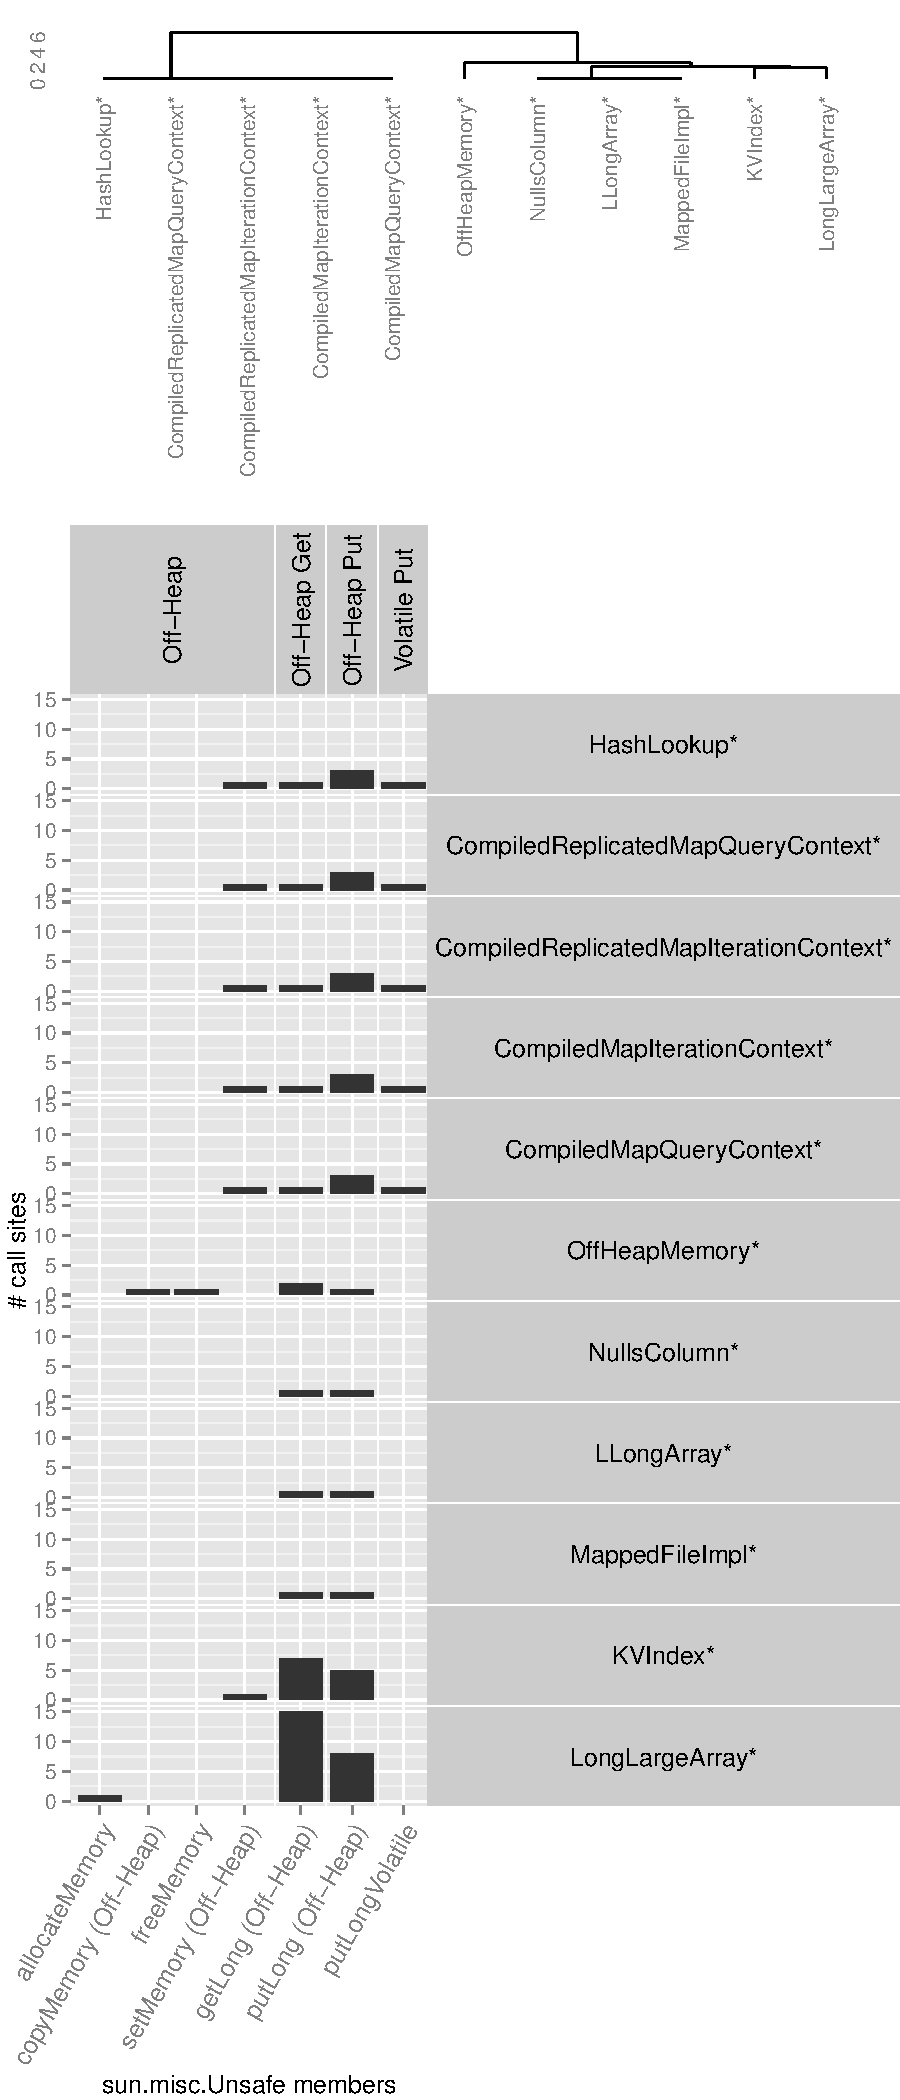
\includegraphics[width=\columnwidth]{chapters/unsafe/classunit}
\caption{Classes using off-heap large arrays}
\label{fig:classunitfingerprint}
\end{figure}

Once we had a clustering of the artifacts by method usage, we manually
inspected a sample of artifacts in each cluster to identify patterns.
Some artifacts contained more than one pattern.
For instance the cluster in Figure~\ref{fig:classunitfingerprint} contains
classes that use \unsafe{} to implement large off-heap arrays, but also
contains
calls to methods of the \smugroup{Put Volatile} group used to implement
strongly shared consistent variables.
We tagged each artifact manually inspected with the set of patterns that it exhibits.
%We have inspected each cluster by 
%--- of the most used artifacts ---
